%% Los cap'itulos inician con \chapter{T'itulo}, estos aparecen numerados y
%% se incluyen en el 'indice general.
%%
%% Recuerda que aqu'i ya puedes escribir acentos como: 'a, 'e, 'i, etc.
%% La letra n con tilde es: 'n.


\chapter{Resultados}

En esta sección se muestran ejemplos de uso tanto del paquete geneticae como de Geneticae Shiny Web APP. 

\section{Paquete de R \emph{geneticae}}

Para instalar la versión del paquete publicada en CRAN: \textcolor{blue}{install.packages}(``geneticae"), mientras que la versión en desarrollo se debe instalar desde el repositorio de Github: devtools::\textcolor{blue}{install\_github}(``jangelini/geneticae"). 

Una vez instalado el paquete, se debe cargar en la sesion de R mediante el comando: \textcolor{blue}{library}(geneticae). 

Información detallada sobre las funciones del paquete geneticae se puede obtener mediante \textcolor{blue}{help}(package = ``geneticae"). La ayuda para una función, por ejemplo \textcolor{blue}{imputation}(), en una sesión R se puede obtener usando \emph{?imputation} o \textcolor{blue}{help}(imputation). La función \textcolor{blue}{browseVignettes}(``geneticae") permite obtener la viñeta del paquete, es decir una descripción el problema que está diseñado para resolver así como ejemplos de aplicación del mismo. 

Además, se encuentra disponible una página web (http://....) que contiene una breve descripción de la utilidad del paquete, las funciones que se incluyen en él, un tutorial de uso, un enlace de acceso a la shiny app, entre otra información.


\subsection{Conjuntos de datos en geneticae}
\label{subsec:datosejemplos}
El paquete geneticae proporciona dos conjuntos de datos que pueden utilizarse para ilustrar la metodología incluida para analizar los datos provenientes de EMA. 

\begin{itemize}[wide, nosep, labelindent = 0pt, topsep = 1ex, noitemsep,topsep=0pt]
\item \emph{yan.winterwheat dataset} \citep{Wright2020}: se cuenta con información sobre el rendimiento de 18 variedades de trigo de invierno cultivadas en nueve ambientes en Ontario en 1993. A pesar de que el experimento contaba con cuatro bloques o réplicas en cada ambiente, sólo el rendimiento medio para cada combinación de variedad y ambiente se encuentra disponible.\\

\begin{tcolorbox}[skin=bicolor,
    colframe=aurometalsaurus,colback=backcolour,colbacklower=white,
    width=1\linewidth,
    height=0.35\linewidth,
    boxsep=-3mm]
\begin{lstlisting}[linewidth=\columnwidth]
data(yan.winterwheat)
head(yanwinterwheat)
\end{lstlisting}

\tcblower\vskip-\baselineskip
\tcblower
\vspace{0.5cm}
\footnotesize\begin{verbatim}
##   gen  env yield
## 1 Ann BH93 4.460
## 2 Ari BH93 4.417
## 3 Aug BH93 4.669
## 4 Cas BH93 4.732
## 5 Del BH93 4.390
## 6 Dia BH93 5.178
\end{verbatim}
\end{tcolorbox}

\item \emph{plrv dataset} \citep{deMendiburu2020} se registró información sobre el rendimiento, el peso de planta y de la parcela de 28 genotipos en 6 localidades de Perú con el fin de estudiar la resistencia a PLRV (\emph{Patato Leaf Roll Virus}) causante del enrollamiento de la hoja. Cada clon fue evaluado tres veces en cada ambiente. \\

\begin{tcolorbox}[skin=bicolor,
    colframe=aurometalsaurus,colback=backcolour,colbacklower=white,
    width=1\linewidth,
    height=0.35\linewidth,
    boxsep=-3mm]
\begin{lstlisting}
data(plrv)
head(plrv)
\end{lstlisting}

\tcblower\vskip-\baselineskip
\tcblower
\vspace{0.5cm}
\footnotesize\begin{verbatim}
##   Genotype Locality Rep WeightPlant WeightPlot    Yield
## 1   102.18     Ayac   1   0.5100000       5.10 18.88889
## 2   104.22     Ayac   1   0.3450000       2.76 12.77778
## 3   121.31     Ayac   1   0.5425000       4.34 20.09259
## 4   141.28     Ayac   1   0.9888889       8.90 36.62551
## 5   157.26     Ayac   1   0.6250000       5.00 23.14815
## 6    163.9     Ayac   1   0.5120000       2.56 18.96296
\end{verbatim}
\end{tcolorbox} 
\end{itemize}
  
  
En las siguiente subsecciones se muestran las herramientas de análisis incluidas en el paquete utilizando el conjunto de datos \emph{yan.winterwheat}.  
  
\subsection{Modelo AMMI}

Para visualizar el efecto de IGA se utiliza el biplot GE obtenido del modelo AMMI. Este gráfico es posible obtenerlo utilizando la función \textcolor{blue}{rAMMI}(). Esta función requiere datos en formato largo, es decir, cada fila corresponde a una observación y cada columna a una variable (genotipo, ambiente, repetición (si existe) y fenotipo observado). Si cada genotipo ha sido evaluado más de una vez en cada ambiente, la media fenotípica para cada combinación de genotipo y ambiente se calcula internamente y luego se estima el modelo. Las variables adicionales que no se utilizarán en el análisis pueden estar presentes en el conjunto de datos. No se permiten valores perdidos pero se pueden imputar como se indica en la subsección \ref{subsec:metimp}. 

El biplot clásico para el conjunto de datos \emph{yan.winterwheat} se muestra en la figura \ref{fig:ammibip} junto con la sentencia utlizada para obtener el mismo. El primer argumento es el conjunto de datos de entrada, luego se indican los nombres de las columnas en las cuales se encuentra la información necesaria para aplicar la técnica y por último el biplot que se desea obtener que por defecto es el derivado del modelo AMMI clásico. Opcionalmente, el porcentaje de IGA explicado por el biplot se puede agregar como una nota al pie con el argumento \emph{footnote = T} así como un título con \emph{titles = T}. 

En este ejemplo, BH93, KE93 y OA93 son los ambientes que más contribuyen a la interacción ya que sus vectores son los de mayor magnitud. Los cultivares m12 y Kat presentan patrones de interacción similares (sus marcadores están próximos entre sí) y son muy diferentes de Ann y Aug, por ejemplo. La cercanía entre el cultivar Dia y el ambiente BH93 indica una fuerte asociación positiva entre ellos, lo que significa que BH93 es un ambiente extremadamente favorable para ese genotipo. Como los marcadores OA93 y Luc son opuestos, este ambiente es considerablemente desfavorable para ese genotipo. Por último, Cas y Reb están cerca del origen, lo que significa que se adaptan en igual medida a todos los ambientes.

\begin{tcolorbox}[skin=bicolor,
    colframe=aurometalsaurus,colback=backcolour,colbacklower=white,
    width=1\linewidth,
    height=0.82\linewidth,
    boxsep=-3mm]
\begin{lstlisting}
rAMMI(yan.winterwheat, genotype = ``gen", environment = ``env", 
      response = ``yield", type = ``AMMI", footnote = F, titles = F)
\end{lstlisting}
\tcblower\vskip-\baselineskip
\tcblower
\begin{figure}[H]
	\begin{center}
		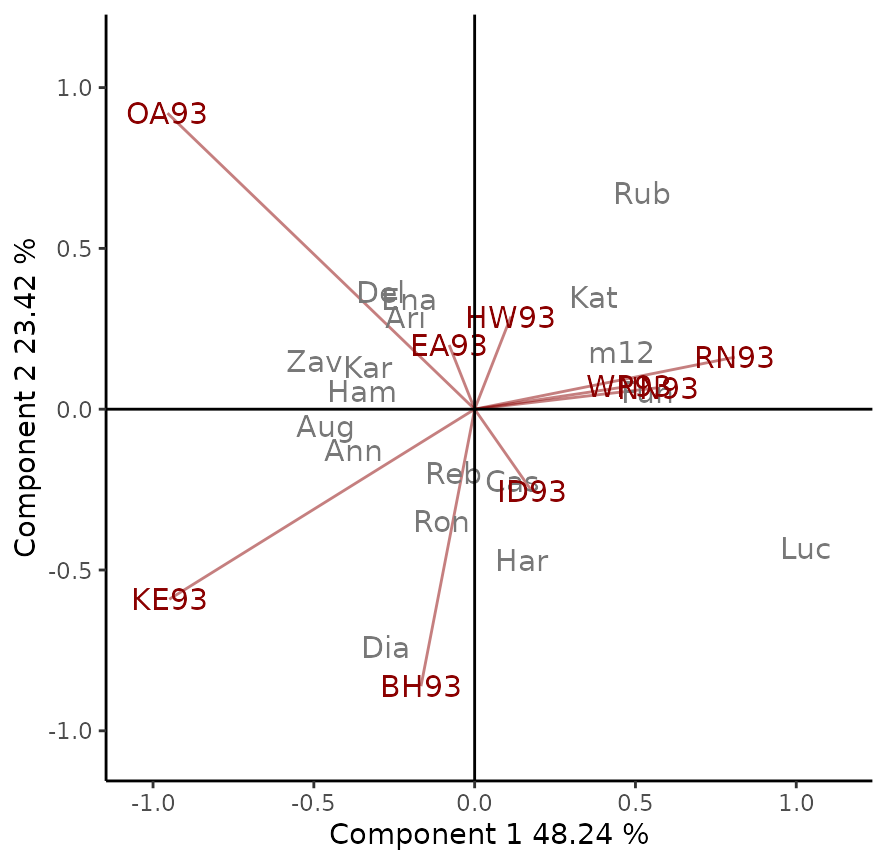
\includegraphics[width=0.80\textwidth]{./Graficos/AMMI_biplot.png}
	\end{center}
	\caption{Biplot GE obtenido del modelo AMMI clásico basado en los datos de rendimiento de trigo de invierno obtenidos en Ontario en 1993. El 71,66\% de la variabilidad de la IGA se explica por los dos primeros términos multiplicativos. Los cultivares se muestran en letras minúsculas y los ambientes en mayúsculas. }
	\label{fig:ammibip}
\end{figure}
\end{tcolorbox}


Como se mencionó anteriormente, el modelo AMMI, en su forma estándar, asume que no hay valores atípicos presentes en los datos. Por lo tanto, en presencia de \emph{outliers} se debe utilizar alguna de las alternativas robustas propuestas por \citet{Rodriguesetal2016}, las cuales no se encuentran disponible en R hasta el momento. Sin embargo, dada la importancia práctica de este reciente avance metodológico, se incluyeron en la función \textcolor{blue}{rAMMI}(). Para obtener los biplots GE derivados de los modelos robustos se debe indicar en el argumento \emph{type} cuál de ellos se desea ajustar: ``rAMMI", ``hAMMI", ``gAMMI", ``lAMMI", ``ppAMMI".

Dado que el conjunto de datos de muestra \emph{yan.winterwheat} no presenta valores atípicos, las conclusiones obtenidas con biplots robustos no diferirán de las obtenidas con el biplot clásico \citep{Rodriguesetal2016}. Por lo tanto, no se presenta ninguna interpretación de los biplots robustos. \\


\subsection{Modelo de Regersión por Sitio}
\label{subsec:SREGpaquete}
Para visualizar conjuntamente el efecto de G e IGA \citet{Yanetal2000} propuso el biplot GGE mediante el cual se pueden abordar diversos aspectos relacionados con la evaluación de genotipos y ambientes. Para obtener dicho biplot en primer lugar se debe ajustar el modelo SREG mediante la función \textcolor{blue}{GGEmodel}(). Ésta es un \emph{wrapper} de \textcolor{blue}{GGEModel}() del paquete GGEBiplots \citep{Dumble2017}. Como en el caso de \textcolor{blue}{rAMMI}(), para poder utilizarla los datos deben presentarse en un formato largo y se permiten repeticiones o variables adicionales en el conjunto de datos. El rasgo fenotípico para cada combinación de genotipo y ambiente debe estar registrado, sino se debe recurrir previamente a alguna técnica de imputación para completar los datos (subsección  \ref{subsec:metimp}). 

La sentencia utilizada para ajustar el modelo GGE en el conjunto de datos \emph{yan.winterwheat} se muestra a continuación. El primer argumento de la misma consiste en el nombre del conjunto de datos y en los siguientes indican los nombres que reciben las columnas que contienen la información de los genotipos, ambientes y del rasgo fenotípico de interés. Por defecto, la función considera que no hay réplicas en el conjunto de datos, sin embargo, si existieran en el parámetro \emph{rep} se debe indicar el nombre de la columna con dicha información. Otros argumentos de dicha función son el método de centrado, de partición de los valores singulares (SVP de sus siglas en ingles \emph{Singular Value Partition}) y escalado. Por defecto los datos se centran utilizando la opción \emph{centering=``tester"} lo cual resulta en el modelo SREG, otro valor dará lugar a un modelo diferente. La elección del método de SVP no altera las relaciones o interacciones relativas entre los genotipos y los ambientes, aunque la apariencia del biplot será diferente (Yan 2002). El método de particion de los valores singulares centrado en los genotipos (\emph{SVP=``row"}) muestra la interrelación entre genotipos con mayor precisión, el enfocado a los ambientes (\emph{SVP=``column"}) es el más informativo de las interrelaciones entre los ambientes, mientras que el simétrico (\emph{SVP=``symmetrical"}) permite visualizar la magnitud relativa tanto de la variación de los genotipos como de los ambientes, por lo que se utiliza por defecto. Por último, se indica que los datos no se deben escalar con el parámetro \emph{scaling=``none"}. \\

\begin{tcolorbox}[colframe=aurometalsaurus,colback=backcolour,colbacklower=white,
   				width=1\linewidth,
    			height=0.12\linewidth,
    			boxsep=-3mm]
\begin{lstlisting}
GGE1 <- GGEmodel(yan.winterwheat, genotype = ``gen", environment = ``env", 
                 response = ``yield", rep = NULL,  centering = ``tester",
  				 scaling = ``none",  SVP = ``symmetrical")
\end{lstlisting}
\end{tcolorbox}


La salida de \textcolor{blue}{GGEModel}() es una lista con los siguientes objetos:
\begin{itemize}
\item coordgenotype: coordenadas para los genotipos en cada componente.
\item coordenviroment: coordenadas para los ambientes en cada componente.
\item eigenvalues: vector de autovalores para cada componente.
\item vartotal: varianza general.
\item varexpl: porcentaje de varianza explicado por cada componente.
\item labelgen: nombres de los genotipos.
\item labelenv: nombres de los ambientes.
\item axes: etiquetas de los ejes.
\item Data: datos escalados y centrados.
\item centering: método de centrado.
\item scaling: método de escala.
\item SVP: método de partición. 
\end{itemize}


Utilizando la salida de \textcolor{blue}{GGEmodel}(), la función 
\textcolor{blue}{GGEPlot}() crea numerosas vistas del biplot GGE que permiten dar respuesta a distintos objetivos de los fitomejoradores. En estos gráficos los cultivares se muestran en minúsculas y los ambientes en mayúsculas. El método de centrado, escalado y SVP se muestran en una nota al pie junto con el porcentaje de G + IGA explicado por los dos ejes al agregar el argumento \emph{footnote = T} y un título con \emph{titles = T}. \\

\textbf{Comparaciones simples utilizando GGE biplot}

El biplot básico se obtiene con el parámetro \emph{type = ``Biplot"} (Figura \ref{fig:ggebip}). En este ejemplo, el 78\% de la variabilidad de G e IGA se explica por los dos primeros términos multiplicativos. Los ángulos entre los marcadores de genotipos y entre los vectores ambientales son utilizados para interpretar el gráfico. Así, por ejemplo, Kat tiene un rendimiento por debajo de la media en todos los ambientes debido a su ángulo superior a $90^{\circ}$ con todos ellos. Por otro lado, Fun presenta un rendimiento superior a la media en todas las localidades excepto OA93 y KE93, como lo indican los ángulos agudos. La longitud de los vectores ambientales es una medida de la capacidad del ambiente para discriminar entre cultivos. 


\begin{tcolorbox}[skin=bicolor,
    colframe=aurometalsaurus,colback=backcolour,colbacklower=white,
    width=1\linewidth,
    height=0.82\linewidth,
    boxsep=-3mm]
\begin{lstlisting}
GGEPlot(GGE1, type = ``Biplot", footnote = F, titles = F)
\end{lstlisting}
\tcblower\vskip-\baselineskip
\tcblower
\begin{figure}[H]
	\begin{center}
		\includegraphics[width=0.80\textwidth]{./Graficos/GGE_biplot.png}
	\end{center}
	\caption{Biplot GGE basado en datos de rendimiento de trigo de invierno obtenido de Ontario en 1993. El método de partición de valores singulares utilizado es el simétrico (opción por defecto). El 78\% de la variabilidad de G + GE se explica por los dos primeros términos multiplicativos. Los cultivares se muestran en minúsculas y los entornos en mayúsculas. }
	\label{fig:ggebip}
\end{figure}
\end{tcolorbox} 

Los mejoradores quieren identificar los cultivares más adaptados a su área, es decir a un ambiente particular, por ejemplo OA93. Para esto, \citet{YanHunt2002} sugieren constituir un eje del ambiente de interés (OA93), trazando una recta que una el identificador del ambiente y el origen de coordenadas, y lo denominan eje OA93. Los genotipos se  clasifican en función del rendimiento en dicho ambiente de acuerdo con sus proyecciones, en la dirección indicada por el eje OA93 (Figura \ref{fig:selectEyG} A). Para obtener esta vista del biplot GGE, se indica la opción \emph{Selected Environment} en el argumento \emph{type} de la función y el ambiente a evaluar en el argumento  \emph{selectedE}. En este ejemplo, el cultivar de mayor rendimiento fue es Zav seguido por Aug, Ham hasta llegar al genotipo Luc, que es el de menor rendimiento en ese ambiente. El eje perpendicular al del ambiente de interés, separa los genotipos con rendimiento mayor al promedio, de Zav a Cas, de aquellos con valores inferior a la media, de Ema a Luc, en OA93.
 
En forma similar, el ambiente más adecuado para un cultivar es posible determinarlo graficando una línea que conecte el origen de coordenadas y el marcador del genotipo de interés, por ejemplo Kat, como se muestra en la figura \ref{fig:selectEyG} B \citep{YanHunt2002}. Los ambientes se clasifican a lo largo del eje del genotipo en la dirección indicada por la flecha. Para obtener este gráfico la opción  \emph{Selected Genotype} debe indicarse en el argumento \emph{type}, y el genotipo de interés en \emph{selectedG}. El eje perpendicular al del genotipo separa los ambientes en los que el cultivar presentó un rendimiento por debajo y por encima del promedio. En este ejemplo, Kat presentó un desempeño por debajo de la media en todos los ambientes estudiados. \\

\begin{tcolorbox}[skin=bicolor,
    colframe=aurometalsaurus,colback=backcolour,colbacklower=white,
    width=1\linewidth,
    height=0.92\linewidth,
    boxsep=-3mm]
\begin{lstlisting}
# Ranking de cultivares en el ambiente OA93
GGEPlot(GGE1, type = ``Selected Environment", selectedE = ``OA93", footnote = F, titles = F)

# Ranking de ambientes para cultivar Kat
GGEPlot(GGE1, type = ``Selected Genotype", selectedG = ``Kat", footnote = F, titles = F)
\end{lstlisting}
\tcblower\vskip-\baselineskip
\tcblower
\begin{figure}[H]
	\begin{center}
		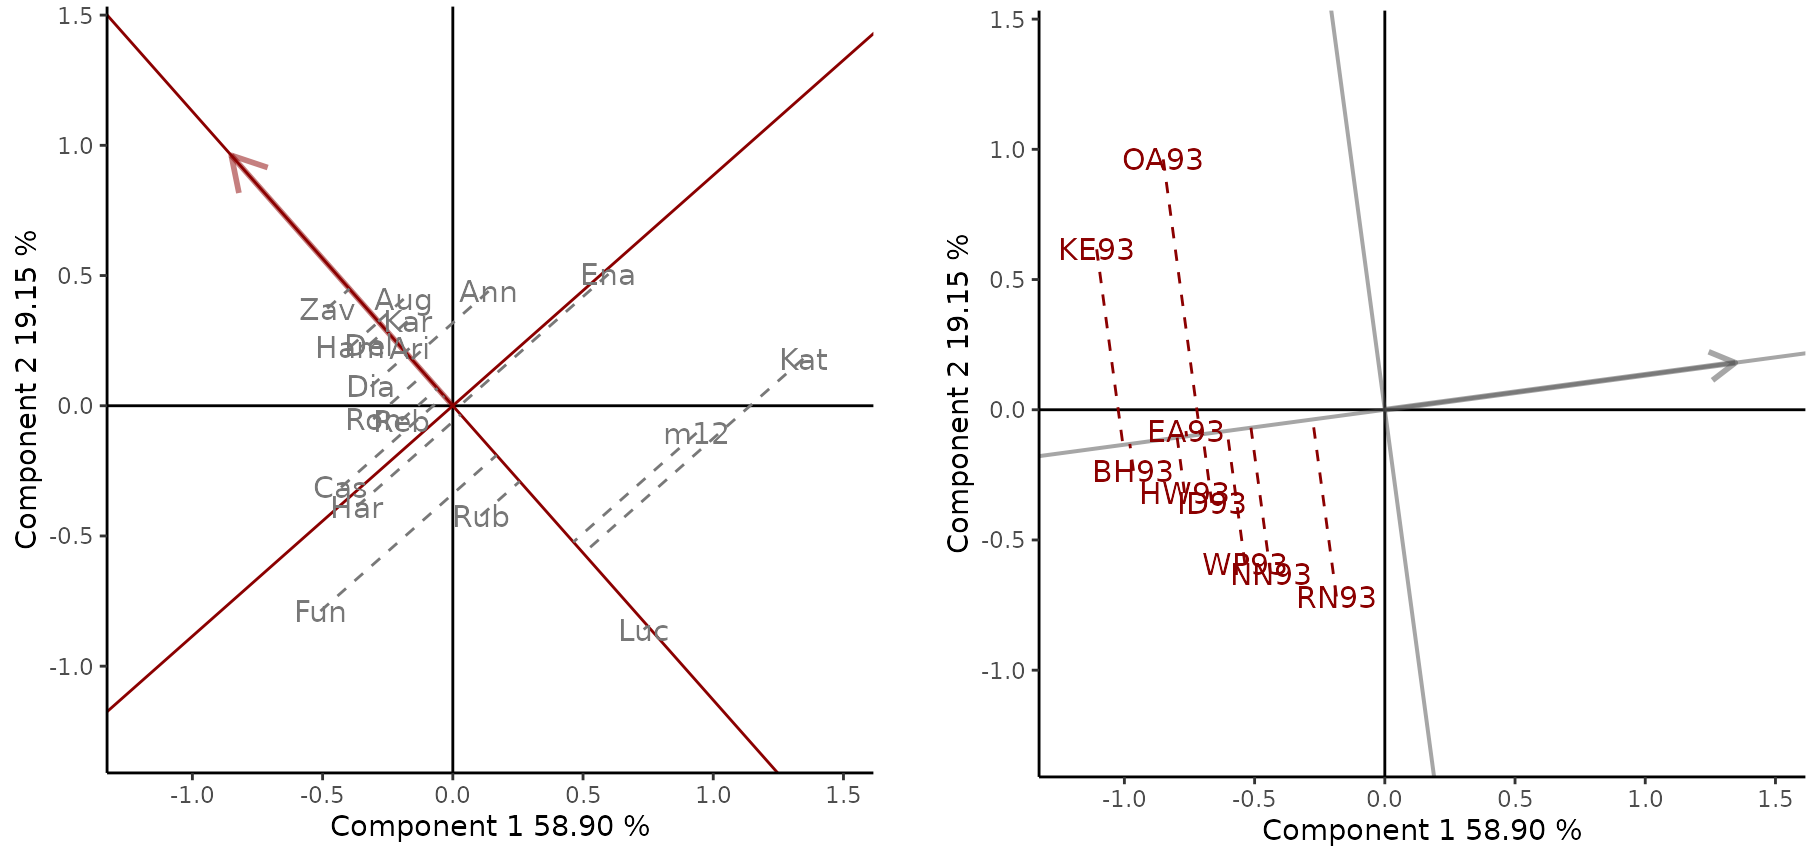
\includegraphics[width=14cm]{./Graficos/SelectedGyE.png}
	\end{center}
	\caption{A: Ranking de cultivares en el ambiente OA93. B: Ranking de ambientes para cultivar Kat, basado en datos de rendimiento de trigo de invierno obtenido de Ontario en 1993. El método de partición de valores singulares utilizado es el simétrico (opción por defecto). El 78\% de la variabilidad de G + GE se explica por los dos primeros términos multiplicativos. Los cultivares se muestran en minúsculas y los entornos en mayúsculas.}
	\label{fig:selectEyG}
\end{figure}
\end{tcolorbox} 


También es posible comparar dos cultivares, por ejemplo Kat y Cas, vinculándolos con una línea y una perpendicular a la anterior (figura \ref{fig:comp2G}). Este biplot se obtiene con \emph{Comparison of Genotype} en el argumento \emph{type} y los genotipos a comparar en \emph{selectedG1} y \emph{selectedG2}. Cas fue más rendidor que Kat en todos los ambientes, ya que todos se ubican en el mismo lado de la línea perpendicular que Cas. 

\begin{tcolorbox}[skin=bicolor,
    colframe=aurometalsaurus,colback=backcolour,colbacklower=white,
    width=1\linewidth,
    height=0.82\linewidth,
    boxsep=-3mm]
\begin{lstlisting}
GGEPlot(GGE1, type = ``Comparison of Genotype", selectedG1 = ``Kat", selectedG2 = ``Cas", footnote = F, titles = F)
\end{lstlisting}
\tcblower\vskip-\baselineskip
\tcblower
\begin{figure}[H]
	\begin{center}
		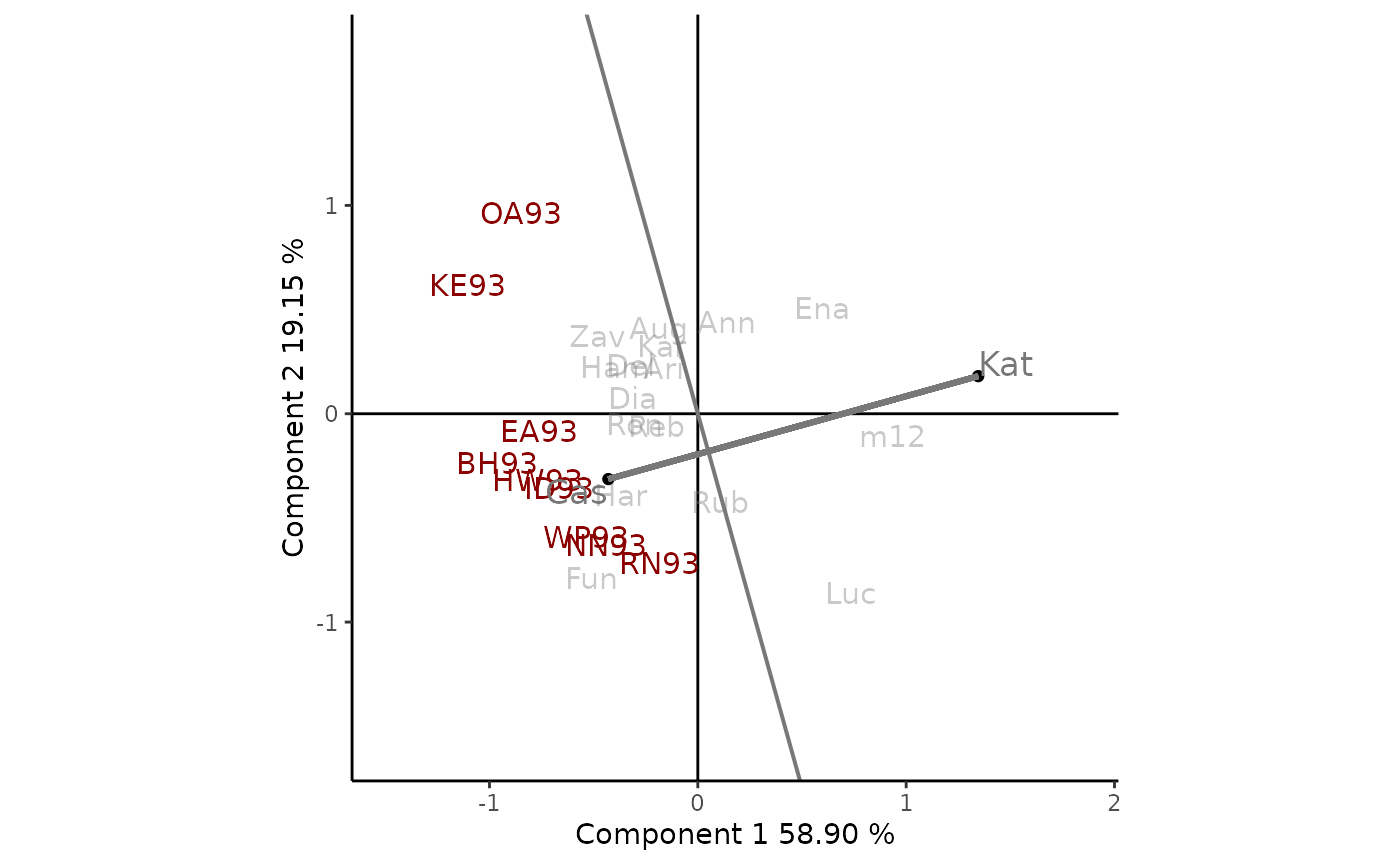
\includegraphics[width=0.80\textwidth]{./Graficos/GGE_comparisonG1yG2.png}
	\end{center}
	\caption{comparación de los cultivares Kat y Cas. El método de partición de valores singulares utilizado es el simétrico (opción por defecto). El 78\% de la variabilidad de G + GE se explica por los dos primeros términos multiplicativos. Los cultivares se muestran en minúsculas y los entornos en mayúsculas. }
	\label{fig:comp2G}
\end{figure}
\end{tcolorbox}


\textbf{Identificación de mega-ambientes con GGE biplot}

La vista poligonal del biplot GGE, obtenida al indicar \emph{Which Won Where/What} en el argumento \emph{type}, proporciona un medio eficaz de visualización del patrón ``quíen ganó dónde"  de un conjunto de datos EMA (Figura \ref{fig:poligono}).  El polígono se obtiene uniendo los cultivares (fun, zav, ena, kat y luc) que se encuentran más alejados del origen de coordenadas, de modo que todos los restantes se encuentren contenidos en el polígono. La distancia de los cultivares respecto del origen de coordenadas, en sus respectivas direcciones, es una medida de la capacidad de respuesta a los ambientes. Los ubicados en los vértices son los más alejados, por lo tanto son los cultivares que más responden, mientras que los que se encuentran en el origen de coordenadas no responden en absoluto a los ambientes estudiados.

Las perpendiculares a los lados del polígono dividen al biplot en mega-ambientes, siendo el cultivar de mayor rendimiento en todos los ambientes que se encuentran en él aquel que se encuentra en el vértice de dicho sector. Por un lado, se observa que OA93 y KE93 conforman un mega-ambiente y que Zav es el mejor cultivar. Otro está formado por el resto de los ambientes, al cual llamaremos ME1 en futuros análisis, siendo Fun el que se encuentra en el vértice. En el sector con ena, kat y luc en los vértices del polígono no se observó ningún ambiente, lo cual indica que estos cultivares fueron los menos rendidores en algunos o todos los ambientes considerados.\\

\begin{tcolorbox}[skin=bicolor,
    colframe=aurometalsaurus,colback=backcolour,colbacklower=white,
    width=1\linewidth,
    height=0.82\linewidth,
    boxsep=-3mm]
\begin{lstlisting}
GGEPlot(GGE1, type = ``Which Won Where/What", footnote = F, titles = F)
\end{lstlisting}
\tcblower\vskip-\baselineskip
\tcblower
\begin{figure}[H]
	\begin{center}
		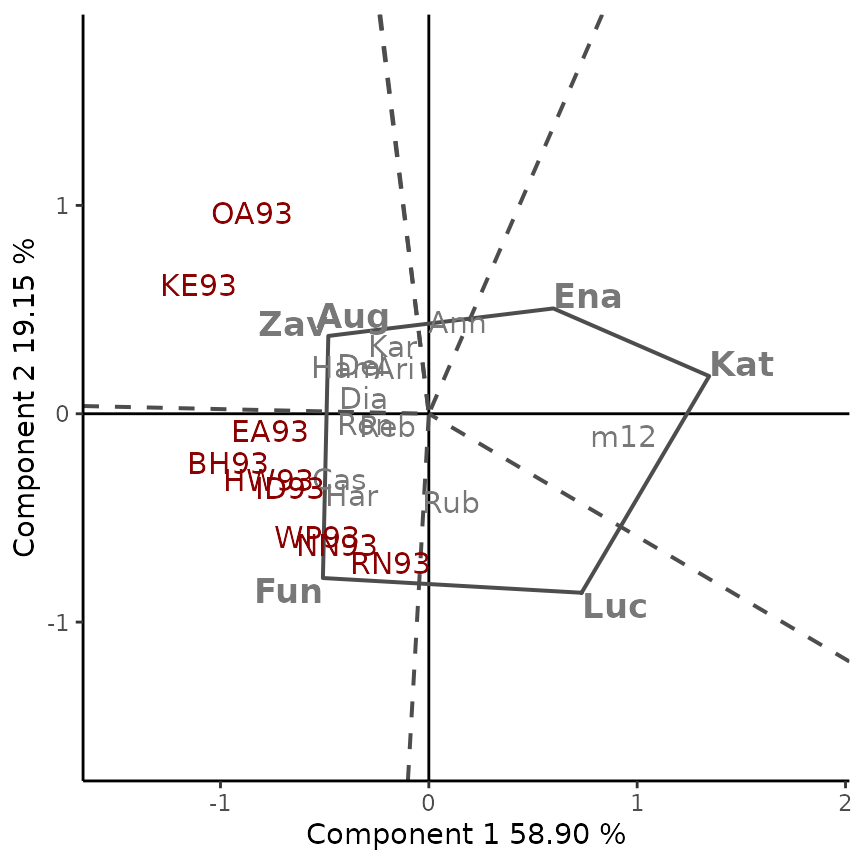
\includegraphics[width=0.80\textwidth]{./Graficos/GGE_whichwonwhere.png}
	\end{center}
	\caption{Vista poligonal del biplot GGE, que muestra qué cultivares presentaron mayor rendimiento en cada ambiente/mega-ambiente. El método de partición de valores singulares utilizado es el simétrico (opción por defecto). El 78\% de la variabilidad de G + GE se explica por los dos primeros términos multiplicativos. Los cultivares se muestran en minúsculas y los entornos en mayúsculas.}
	\label{fig:poligono}
\end{figure}
\end{tcolorbox}

\textbf{Evaluación de los cultivos dentro de un mega-ambientes con GGE biplot}

Una vez identificado los mega-ambientes, el siguiente paso es seleccionar cultivares dentro de cada uno de ellos. De acuerdo con la figura  \ref{fig:poligono}, zav es el mejor cultivar para los ambientes en uno de los mega-ambiente y fun para el otro. Sin embargo, los fitomejoradores no seleccionarán un único cultivar en cada mega-ambiente, sino que es necesario evaluar todos los cultivares con el fin de conocer su desempeño (rendimiento y estabilidad).  

El biplot GGE, particularmente utilizando el factor de partición de la descomposición en valores singulares enfocando en los genotipos, es decir utilizando el argumento \emph{SVP=``row"} en la función \textcolor{blue}{GGEmodel}(), proporciona un medio superior para visualizar tanto el rendimiento medio como la estabilidad de los genotipos (Figura \ref{fig:evaluacionG}). Esto se debe a que la unidad de ambos ejes para los genotipos es la unidad original de los datos. Además, dado que el interés radica en los genotipos y no en los ambientes, se indica con el argumento \emph{sizeEnv = 0} de la función \textcolor{blue}{GGEPlot}() para que no se los muestre en el gráfico.


La visualización del rendimiento medio y la estabilidad de los genotipos se logra dibujando una coordenada ambiental promedio (AEC, por sus siglas en inglés \emph{Average environment coordination}). Por ejemplo, la Figura \ref{fig:evaluacionG}  muestra el AEC para el megaambiente ME1 compuesto por los entornos BH93, EA93, HW93, ID93, NN93, RN93, WP93. Mientras que la abscisa representa el efecto de G la ordenada el de la IGA, que es una medida de la variabilidad o inestabilidad, asociada con cada genotipo. Una mayor proyección sobre la ordenada AEC, independientemente de la dirección, significa mayor inestabilidad. Fun fue claramente el cultivar de mayor rendimiento, en promedio, en este megaambiente, seguido por Cas y Har, y Kat fue el más pobre. Mientras que Rub y Dia son más variables y menos estables que otros cultivares, por el contrario, Cas, Zav, Reb, Del, Ari y Kar, fueron más estables. 

La Figura \ref{fig:evaluacionG} compara los cultivares con el ``ideal” que es el más rendidor y con estabilidad absoluta. Este cultivar ideal se usa como referencia, ya que rara vez existe. La distancia entre los cultivares y el ideal se puede utilizar como medida de conveniencia. Los círculos concéntricos ayudan a visualizar estas distancias. En el ejemplo, para el ME1, Fun es el más cercano al cultivo ideal, y por tanto el más deseable, seguido de Cas y Har, y Kat fue el más lejano. \\

\textbf{FALTAEL SIGNO \$ EN LA PRIMER LINEA DEL CODIGO QUE SIGUE...PERO ME TIRA ERROR O PONERLO CON FILTER???}

\begin{tcolorbox}[skin=bicolor,
    colframe=aurometalsaurus,colback=backcolour,colbacklower=white,
    width=1\linewidth,
    height=1.1\linewidth,
    boxsep=-3mm]
\begin{lstlisting}

ME1 <- yan.winterwheat[yan.winterwheat env %in% c(``BH93", ``EA93",``HW93", ``ID93",``NN93", ``RN93", ``WP93"), ]
                                                   
# Modelo SREG enfocando SVD en los genotipos
GGE_Gpartition <- GGEmodel(ME1, genotype = ``gen", environment = ``env", response = ``yield", SVP = ``row")

# Visualizacion del rendimiento medio y la estabilidad
GGEPlot(GGE_Gpartition, type = ``Mean vs. Stability", footnote = F, titles = F, sizeEnv = 0)

# Ranking de los genotipos respecto a uno ideal
GGEPlot(GGE_Gpartition, type = ``Ranking Genotypes", footnote = F, titles = F, sizeEnv = 0)

\end{lstlisting}
\tcblower\vskip-\baselineskip
\tcblower
\begin{figure}[H]
	\begin{center}
		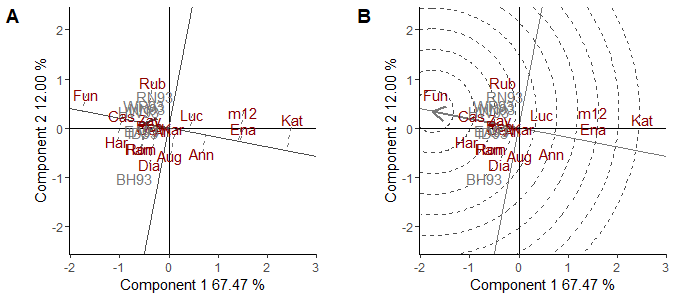
\includegraphics[width=14cm]{./Graficos/MeanvsStability2.png}
	\end{center}
	\caption{A: Evaluación de los cultivares con base en el rendimiento promedio y la estabilidad y B: Clasificación de genotipos con respecto al genotipo ideal, basado en el método de patición de la descomposición en valores singulares enfocado en los genotipos.}
	\label{fig:evaluacionG}
\end{figure}
\end{tcolorbox}


\textbf{Evaluación de los ambientes con GGE biplot}

A pesar de que el objetivo principal de los EMA es seleccionar cultivares también es posible evaluar los ambientes. Esto incluye varios aspectos: (i) evaluar si la región objetivo pertenece a uno o más megaambientes; (ii) identificar mejores entornos de prueba; (iii) detectar ambientes redundantes que no brindan información adicional sobre cultivares; y (iv) determinar los ambientes que se pueden utilizar para la selección indirecta. Para ello, se enfoca la partición de los valores singulares en los ambientes al ajustar el modelo SREG (\emph{SVP = ``column"} en la función \textcolor{blue}{GGEmodel}()). 

En la figura \ref{fig:evaluacionE} los ambientes están conectados con el origen de coordenadas a través de vectores, permitiendo comprender las interrelaciones entre ellos.  Esta visualización del biplot GGE se obtiene indicando \emph{Relationship Among Environments} (Figura \ref{fig:evaluacionE}) en el parámetro \emph{type}. El coeficiente de correlación entre dos ambientes es aproximadamente el coseno del ángulo entre sus vectores. 
En este ejemplo se considera la relación entre los ambientes de ME1. El ángulo entre los vectores para los entornos NN93 y WP93 es de aproximadamente $10^{\circ}$ entre sus vectores; por lo tanto, están estrechamente relacionados; mientras que RN93 y OA93 presentan una correlación negativa débil ya que el ángulo es levemente mayor a $90^{\circ}$. El coseno de los ángulos no se traduce precisamente en coeficientes de correlación, ya que el biplot no explica toda la variabilidad en el conjunto de datos. Sin embargo, son lo suficientemente informativos como para comprender la interrelación entre los entornos de prueba. 

Si algunos de los ambientes tienen ángulos pequeños y, por lo tanto, están altamente correlacionados, la información sobre los genotipos obtenidos de estos ambientes debe ser similar. Si esta similitud es repetible a través de los años, estos ambientes son redundantes y por lo tanto, uno solo debería ser suficiente. Obtener la misma o mejor información utilizando menos ambientes reducirá el costo y aumentará la eficiencia de producción.


La capacidad de discriminación así como la representatividad respecto del ambiente objetivo, son medidas fundamentales para un ambiente. Si no tiene capacidad de discriminación, no proporciona información sobre los cultivares y, por lo tanto, carece de utilidad. A su vez, si no es representativo no sólo que carece de utilidad sino que también puede proporcionar información sesgada sobre los cultivares evaluados. Para visualizar estas medidas, se define una coordenada ambiental promedio (AEC mencionado anteriormente) y el ambiente ideal como el centro de un conjunto de círculos concéntricos (Figura \ref{fig:evaluacionE}). Para obtener este biplot se debe indicar \emph{Ranking Environments} en el argumento \emph{type} de \textcolor{blue}{GGEPlot}() (Figura \ref{fig:evaluacionE}). El ángulo entre el vector de un ambiente y el eje proporciona una medida de la representatividad. Por lo tanto, EA93 e ID93 son los más representativos, mientras que RN93 y BH93 son los menos representativos del ambiente promedio, cuando se analiza ME1. Por otro lado, para ser discriminativo debe estar cercano al ambiente ideal. HW93 es el ambiente más cercano al ideal y, por lo tanto, es el más deseable del ME1, seguido por EA93 e ID93. Por el contrario, RN93 y BH93 fueron los ambientes de prueba menos deseables de ME1. 

\begin{tcolorbox}[skin=bicolor,
    colframe=aurometalsaurus,colback=backcolour,colbacklower=white,
    width=1\linewidth,
    height=0.885\linewidth,
    boxsep=-3mm]
\begin{lstlisting}
# Modelo SREG enfocando SVD en los ambientes
GGE_Epartition <- GGEmodel(ME1, genotype=``gen", environment=``env", response=``yield", SVP=``column")

# Relacion entre ambientes
GGEPlot(GGE_Epartition, type = ``Relationship Among Environments", footnote = F, titles = F)

# Clasificacion de ambientes con respecto al ambiente ideal
GGEPlot(GGE_Epartition, type = ``Ranking Environments", footnote = F, titles = F)
\end{lstlisting}
\tcblower\vskip-\baselineskip
\tcblower
\begin{figure}[H]
	\begin{center}
		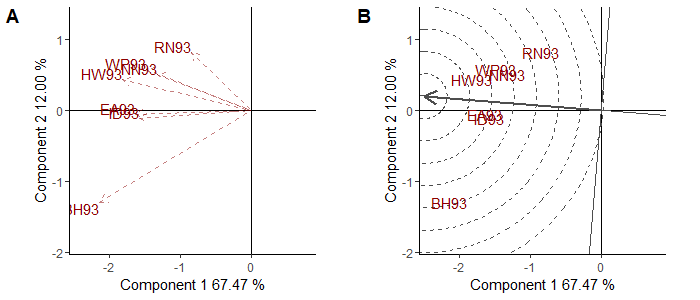
\includegraphics[width=14cm]{./Graficos/RelationshipEnvironments.png}
	\end{center}
	\caption{A: Relación entre ambientes y B: Clasificación de ambientes con respecto al ambiente ideal, basado en el escalado centrado en los genotipos.}
	\label{fig:evaluacionE}
\end{figure}
\end{tcolorbox}


\subsection{Métodos de imputación}
\label{subsec:metimp}

Una limitación importante de los modelos presentados anteriormente es que requieren que el conjunto de datos este completo, es decir que todos los genotipos sean evaluados en todos los ambientes. Por lo tanto, en el paquete se incluyen una serie de metodologías de imputación desarrolladas específicamente para datos genotipo-ambiente recientemente publicadas, algunas de las cuales no se encuentran disponible en R, para superar el problema de las observaciones perdidas. Entre los métodos incluidos se encuentran: ``EM-AMMI", ``EM-SVD", ``Gabriel",``WGabiel"  y ``EM-PCA", los cuales se indican en la opción \emph{type} de la función \textcolor{blue}{imputation}(). El formato requerido para el conjunto de datos de entrada es análogo al indicado en las otras funciones incluidas en el paquete. 

Para presentar un ejemplo, se eliminan algunas observaciones del conjunto de datos \emph{yan.winterwheat} ya que contaba con todos los registros completos:

\begin{tcolorbox}[skin=bicolor,
    colframe=aurometalsaurus,colback=backcolour,colbacklower=white,
    width=1\linewidth,
    height=0.15\linewidth,
    boxsep=-3mm]
\begin{lstlisting}
# Generando datos faltantes
yan.winterwheat [1,3] <- NA
yan.winterwheat [3,3] <- NA
yan.winterwheat [2,3] <- NA
\end{lstlisting}
\end{tcolorbox}

La imputación de valores perdidos con el método ``EM-AMMI" se puede realizar de la siguiente manera:

\begin{tcolorbox}[skin=bicolor,
    colframe=aurometalsaurus,colback=backcolour,colbacklower=white,
    width=1\linewidth,
    height=0.1\linewidth,
    boxsep=-3mm]
\begin{lstlisting}
imputation(yanwinterwheat, PC.nb = 2, genotype = ``gen", environment = ``env", response = ``yield", type = ``EM-AMMI")
\end{lstlisting}
\end{tcolorbox}

El resultado es la matriz con datos imputados en aquellas celdas vacías. 


\section{Geneticae Shiny Web App}

El objetivo de Geneticae Shiny Web APP es proporcionar una interfaz gráfica de usuario para el paquete geneticae de R descripto anteriormente, de modo que pueda ser utilizado por fitomejoradores y analistas sin experiencia previa en programación R. 

Es un software interactivo, no comercial y de código abierto, que ofrece una alternativa gratuita al software comercial disponible para analizar datos provenientes de ensayos multiambientales. Se encuentra disponible en un servidor gratiuto \url{https://geneticae.shinyapps.io/geneticae-shiny-web-app/} el cual tiene límite en el tiempo de uso, sin embargo, la APP será ubicada en el servidor de CONICET para su libre navegación. Además, se puede acceder a la misma desde la página web del instituto CEFOBI de CONICET \url{https://www.cefobi-conicet.gov.ar/bases-de-datos-y-programas/}.

En las subsecciones siguientes se presentará un ejemplo de cómo cargar y analizar datos con la aplicación.


\subsection{Preparación de un archivo de datos}

La APP requiere que los datos de entrada se encuentren en formato .csv, delimitados por comas, punto y coma o tabulaciones. Los nombres de las columnas pueden ubicarse en la primera fila del archivo (\emph{heading}). Los datos deben estar en formato largo, es decir, cada fila corresponde a una observación y cada columna a una variable (genotipo, ambiente, repetición (si existe) y fenotipo observado). Si cada genotipo ha sido evaluado más de una vez en cada ambiente, la media fenotípica requerida por el modelo SREG y AMMI para cada combinación de genotipo y ambiente se calcula internamente antes de ajustar dichos modelos. Las variables adicionales que no se utilizarán en el análisis pueden estar presentes en el conjunto de datos. No se permiten valores perdidos.

Los dos conjuntos de datos \emph{plrv} y \emph{yanwinterwheat} descriptos en la subsección \ref{subsec:datosejemplos} están disponibles en la pestaña \emph{Data $->$ Example datasets} y se pueden descargar en formato .csv (Figura \ref{fig:dataexample}) para poder seguir el tutorial de uso de la APP. El conjunto de datos \emph{yanwinterwheat} no tiene repeticiones, mientras que \emph{plrv} sí. 

 \begin{figure}[H]
	\begin{center}
		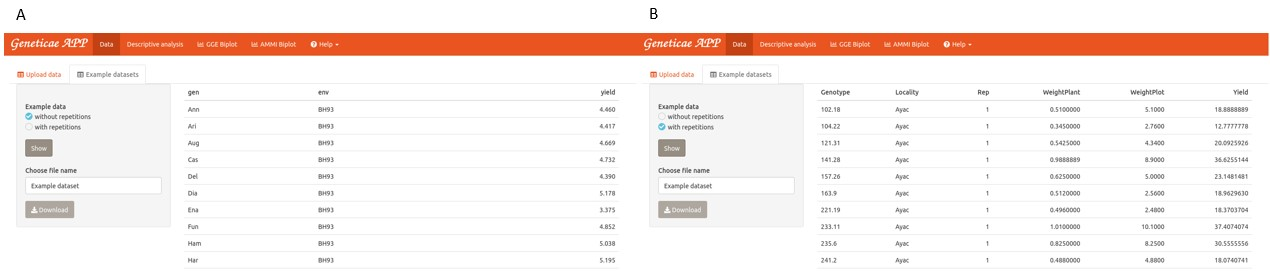
\includegraphics[width=0.8\textwidth]{./Graficos/www/exampledata.jpg}
	\end{center}
	\caption{(A) Plrv dataset (B) yanwinterwheat dataset }
	\label{fig:dataexample}
\end{figure}

En los ejemplos que continuan se utilizará el conjunto de datos \emph{yanwinterwheat}.

\textbf{Cargando un conjunto de datos en la APP}

El conjunto de datos que se analizará debe cargarse en la pestaña \emph{Data $->$ Upload data}. Por ejemplo, para importar el conjunto de datos \emph{yanwinterwheat}, se debe cargar el archivo .csv. Una vez cargado, se debe indicar que está delimitado por comas, que la primera fila contiene los nombres de cada variable (\emph{heading}) y los nombres de las columnas que continen la información del genotipo, ambiente y rasgo fenotípico (gen, env y rendimiento en este ejemplo). Si hay repeticiones disponibles, se debe especificar el nombre de la columna con dicha información; de lo contrario, el campo queda vacío. 

 \begin{figure}[H]
	\begin{center}
		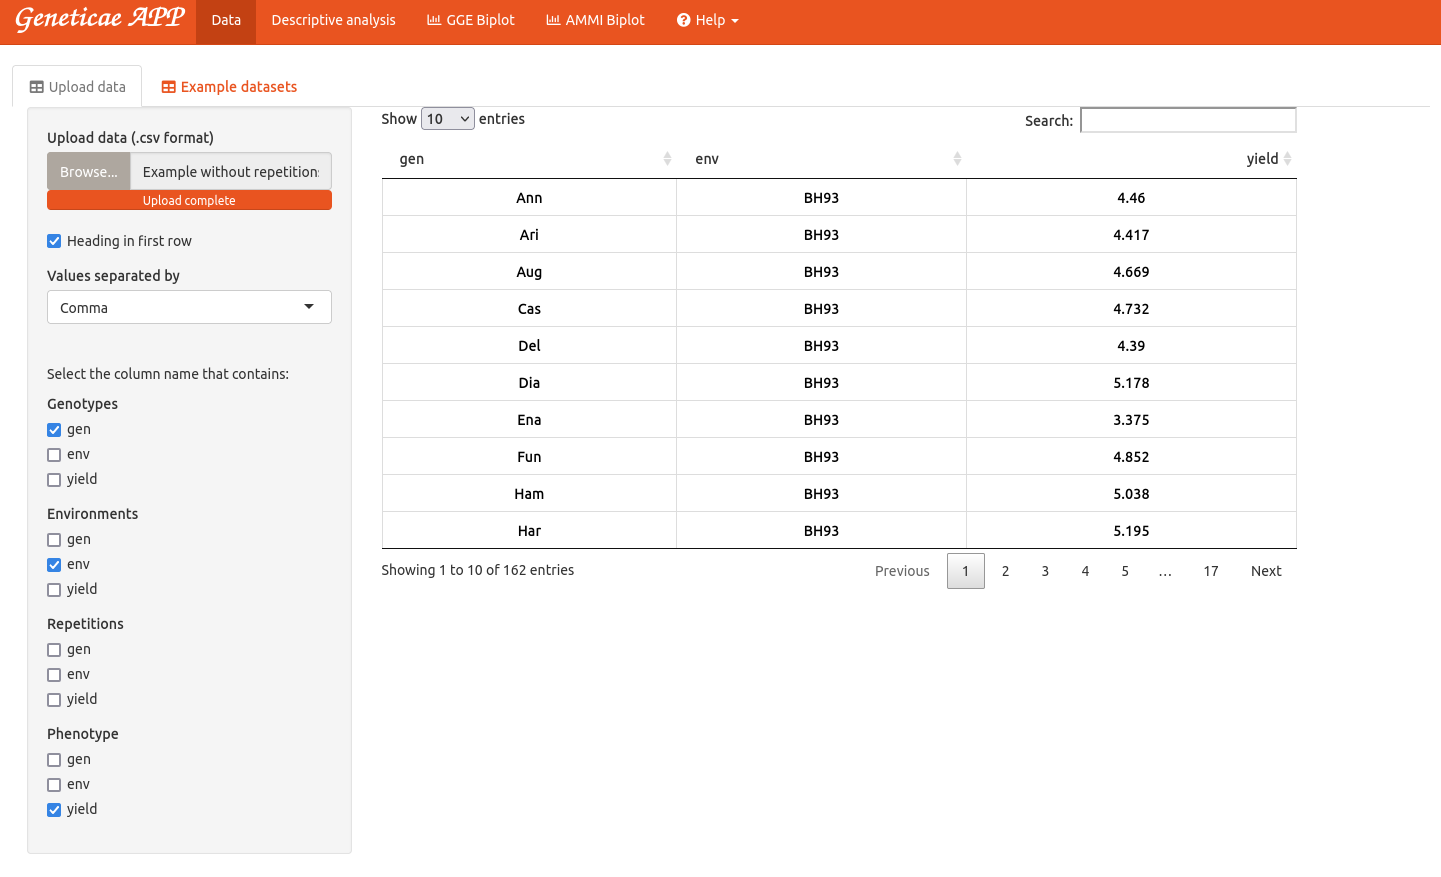
\includegraphics[width=16cm]{./Graficos/www/Data.png}
	\end{center}
	\caption{Cargando el conjunto de datos \emph{yanwinterwheat} en Geneticae APP}
	\label{fig:fig431}
\end{figure}


\subsection{Análisis descriptivo}

Cualquier estudio debe comenzar con un análisis descriptivo del conjunto de datos. La pestaña \emph{Descriptive Analysis} proporciona algunas herramientas para esto, como  \emph{boxplot}, diagrama y matriz de correlación así como también gráficos de interacción.

Un \emph{boxplot} que compara el rasgo cuantitativo entre ambientes o genotipos puede ser de interés (Figura \ref{fig:figdesc1}). Las medidas de resumen utilizadas para su construcción se muestran de forma interactiva moviendo el mouse dentro del panel de la figura. Además, se puede descargar como un archivo .png o en forma interactiva (.html), haciendo clic en la cámara que aparece en la figura o en el botón Descargar, respectivamente. El usuario puede personalizar algunos aspectos del gráfico, como el color de las cajas y los nombres de los ejes. 

\begin{figure}[H]
	\begin{center}
		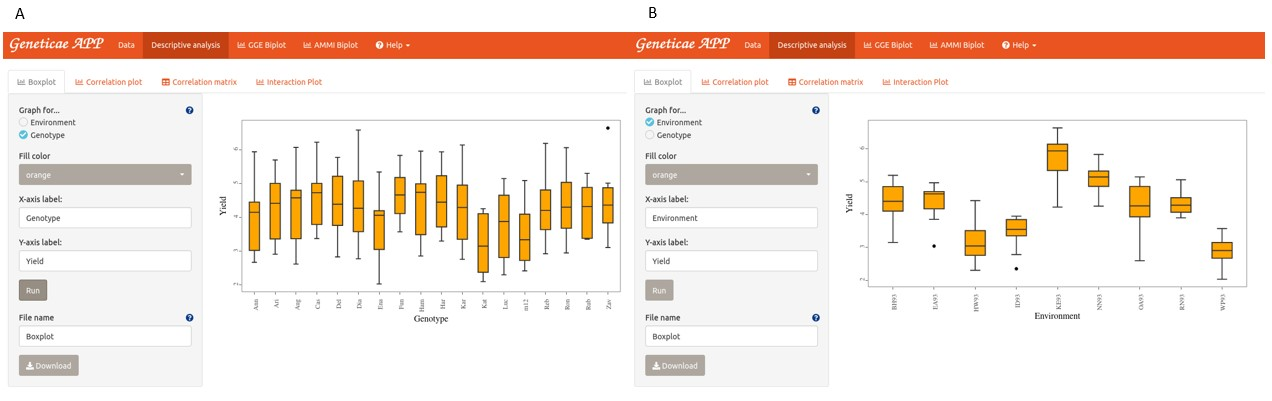
\includegraphics[width=16cm]{./Graficos/Boxplot.jpg}
	\end{center}
	\caption{Diagrama de caja de (A) genotipos y (B) ambientes para el conjunto de datos \emph{yanwinterwheat}.}
	\label{fig:figdesc1}
\end{figure}

Los coeficientes de correlación de Pearson o Spearman entre genotipos se pueden mostrar como un gráfico o una matriz (Figura \ref{fig:figdesc2}). Gráficamente, las correlaciones positivas se muestran en azul y las negativas en rojo, mientras que la intensidad del color y el tamaño del círculo son proporcionales a la magnitud de los coeficientes de correlación. La gráfica de correlación se puede descargar en formato .png. Se observan altas correlaciones entre el rendimiento de los genotipos estudiados. 

\begin{figure}[H]
	\begin{center}
		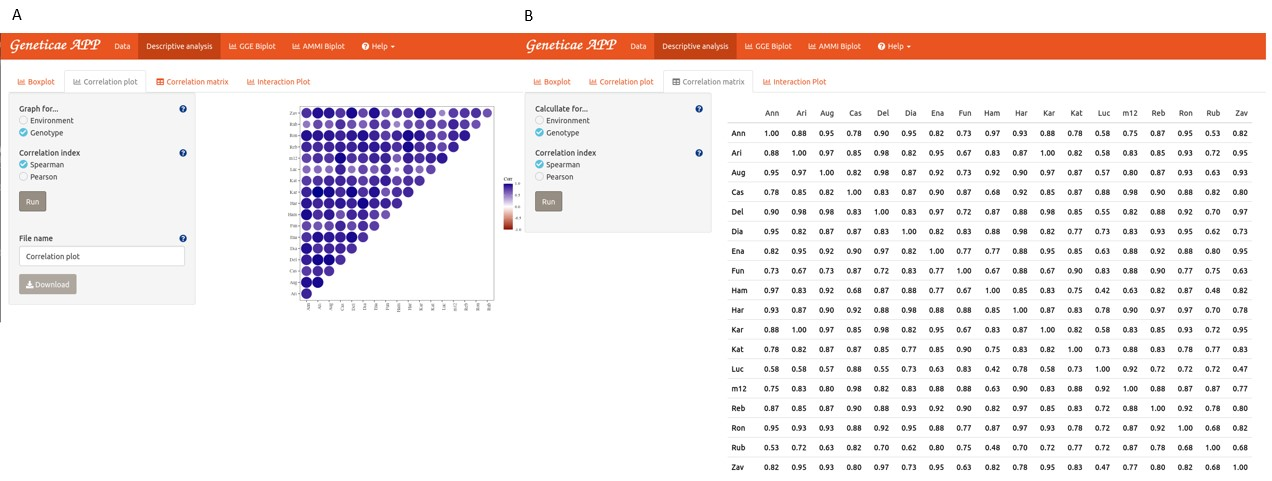
\includegraphics[width=16cm]{./Graficos/correlacion.jpg}
	\end{center}
	\caption{Gráfico de correlación (A) y matriz (B) entre genotipos yanwinterwheat dataset }
	\label{fig:figdesc2}
\end{figure}


Dado que IGA genera respuestas genotípicas diferenciales en diferentes ambientes, lo que complica selección de los mejores cultivares, una gráfico de interacción puede ser de interés (Figura \ref{fig:figdesc3}). El cambio en el efecto genotípico a través de los ambientes se muestra en la figura \ref{fig:figdesc3} A, mientras que el cambio en el efecto ambiental a través de los genotipos en la figura \ref{fig:figdesc3} B. Del mismo modo que el \emph{boxplot} es un gráfico interactivo, por lo que es posible descargarla en formatos .HTML o .png con el botón Descargar o haciendo clic en la cámara, respectivamente. Además, el usuario puede personalizar los nombres de los ejes. En este ejemplo se pueden ver inconsistencias en el desempeño de genotipos en diferentes ambientes. 


\begin{figure}[H]
	\begin{center}
		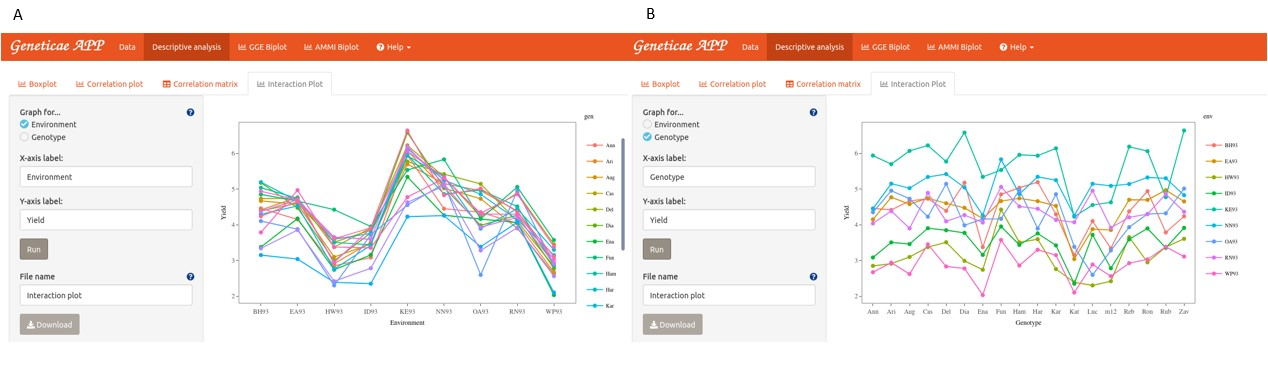
\includegraphics[width=16cm]{./Graficos/interaction.jpg}
	\end{center}
	\caption{Gráfico de interacción para (A) ambientes a través de genotipos y (B) genotipos a través de entornos del conjunto de datos de \emph{yanwinterwheat}.}
	\label{fig:figdesc3}
\end{figure}


\subsection{Modelo de regresión por sitio}

\emph{Geneticae Shiny Web App} permite generar las vistas del biplot GGE presentados en la subsección \ref{subsec:SREGpaquete} mediante la pestaña \emph{GGE Biplot}. Del mismo modo que en el paquete geneticae, los cultivares se presentan en minúsculas y los ambientes en mayúsculas. Dado que el modelo SREG requiere una única observación para cada combinación de genotipo y ambiente, si hay repeticiones, el valor fenotípico promedio se calcula automáticamente antes de ajustar el modelo. No se permiten valores perdidos. 

Se debe seleccionar el método de partición de los valores singulares (\emph{SVP type}) sin embargo, como se mencionó anteriormente esta elección no altera las relaciones o interacciones relativas entre genotipos y ambientes, aunque la apariencia del biplot será diferente (Yan, 2002). La opción simétrica permite la comparación tanto de genotipos como de ambientes (opción por \emph{default}); \emph{Genotype-Focused} muestra la interrelación entre genotipos con mayor precisión que cualquier otro método, y \emph{Environment-Focused} es la que más informa sobre las interrelaciones entre ambientes. Una nota a pie del gráfico que indica que el método de centrado, que será siempre \emph{tester-center} para obtener el biplot GGE, que no se aplica ninguna escala a los datos, el método SVP seleccionado por el usuario y el porcentaje de variación de G e IGA explicado por los dos ejes puede ser agregado. A su vez, el título del gráfico, los ejes y los nombres de los mismos se pueden configurar para que aparezcan o no. Por último, ciertos atributos estilísticos de dichos gráficos se pueden personalizar como el color y tamaño de los marcadores de genotipos y ambientes, y además los gráficos pueden ser descargados.  

El biplot básico, la vista del biplot GGE que muestra los cultivares más adecuados para un ambiente particular (OA93), los ambientes más adecuados para un genotipo (Kat), la comparación de dos genotipos (Cas y Kat) y la vista del poligono se pueden obtener como se indica en la figura \ref{fig:ggebip1}, donde el escalado es el simétrico (\emph{SVP type $->$ symmetrical}) y las opciones de \emph{plot type} son \emph{Biplot,
Selected Environment, Selected Genotype, Comparison of Genotype} y \emph{Which Won Where/What}, respectivamente. Al indicar \emph{Selected Environment} el ambiente de interés se debe especificar, de igual modo cuando se utiliza \emph{Selected Genotype} y 
\emph{Comparison of Genotype} se debe señalar cuál es el genotipo a analizar.

\begin{figure}[H]
	\begin{center}
		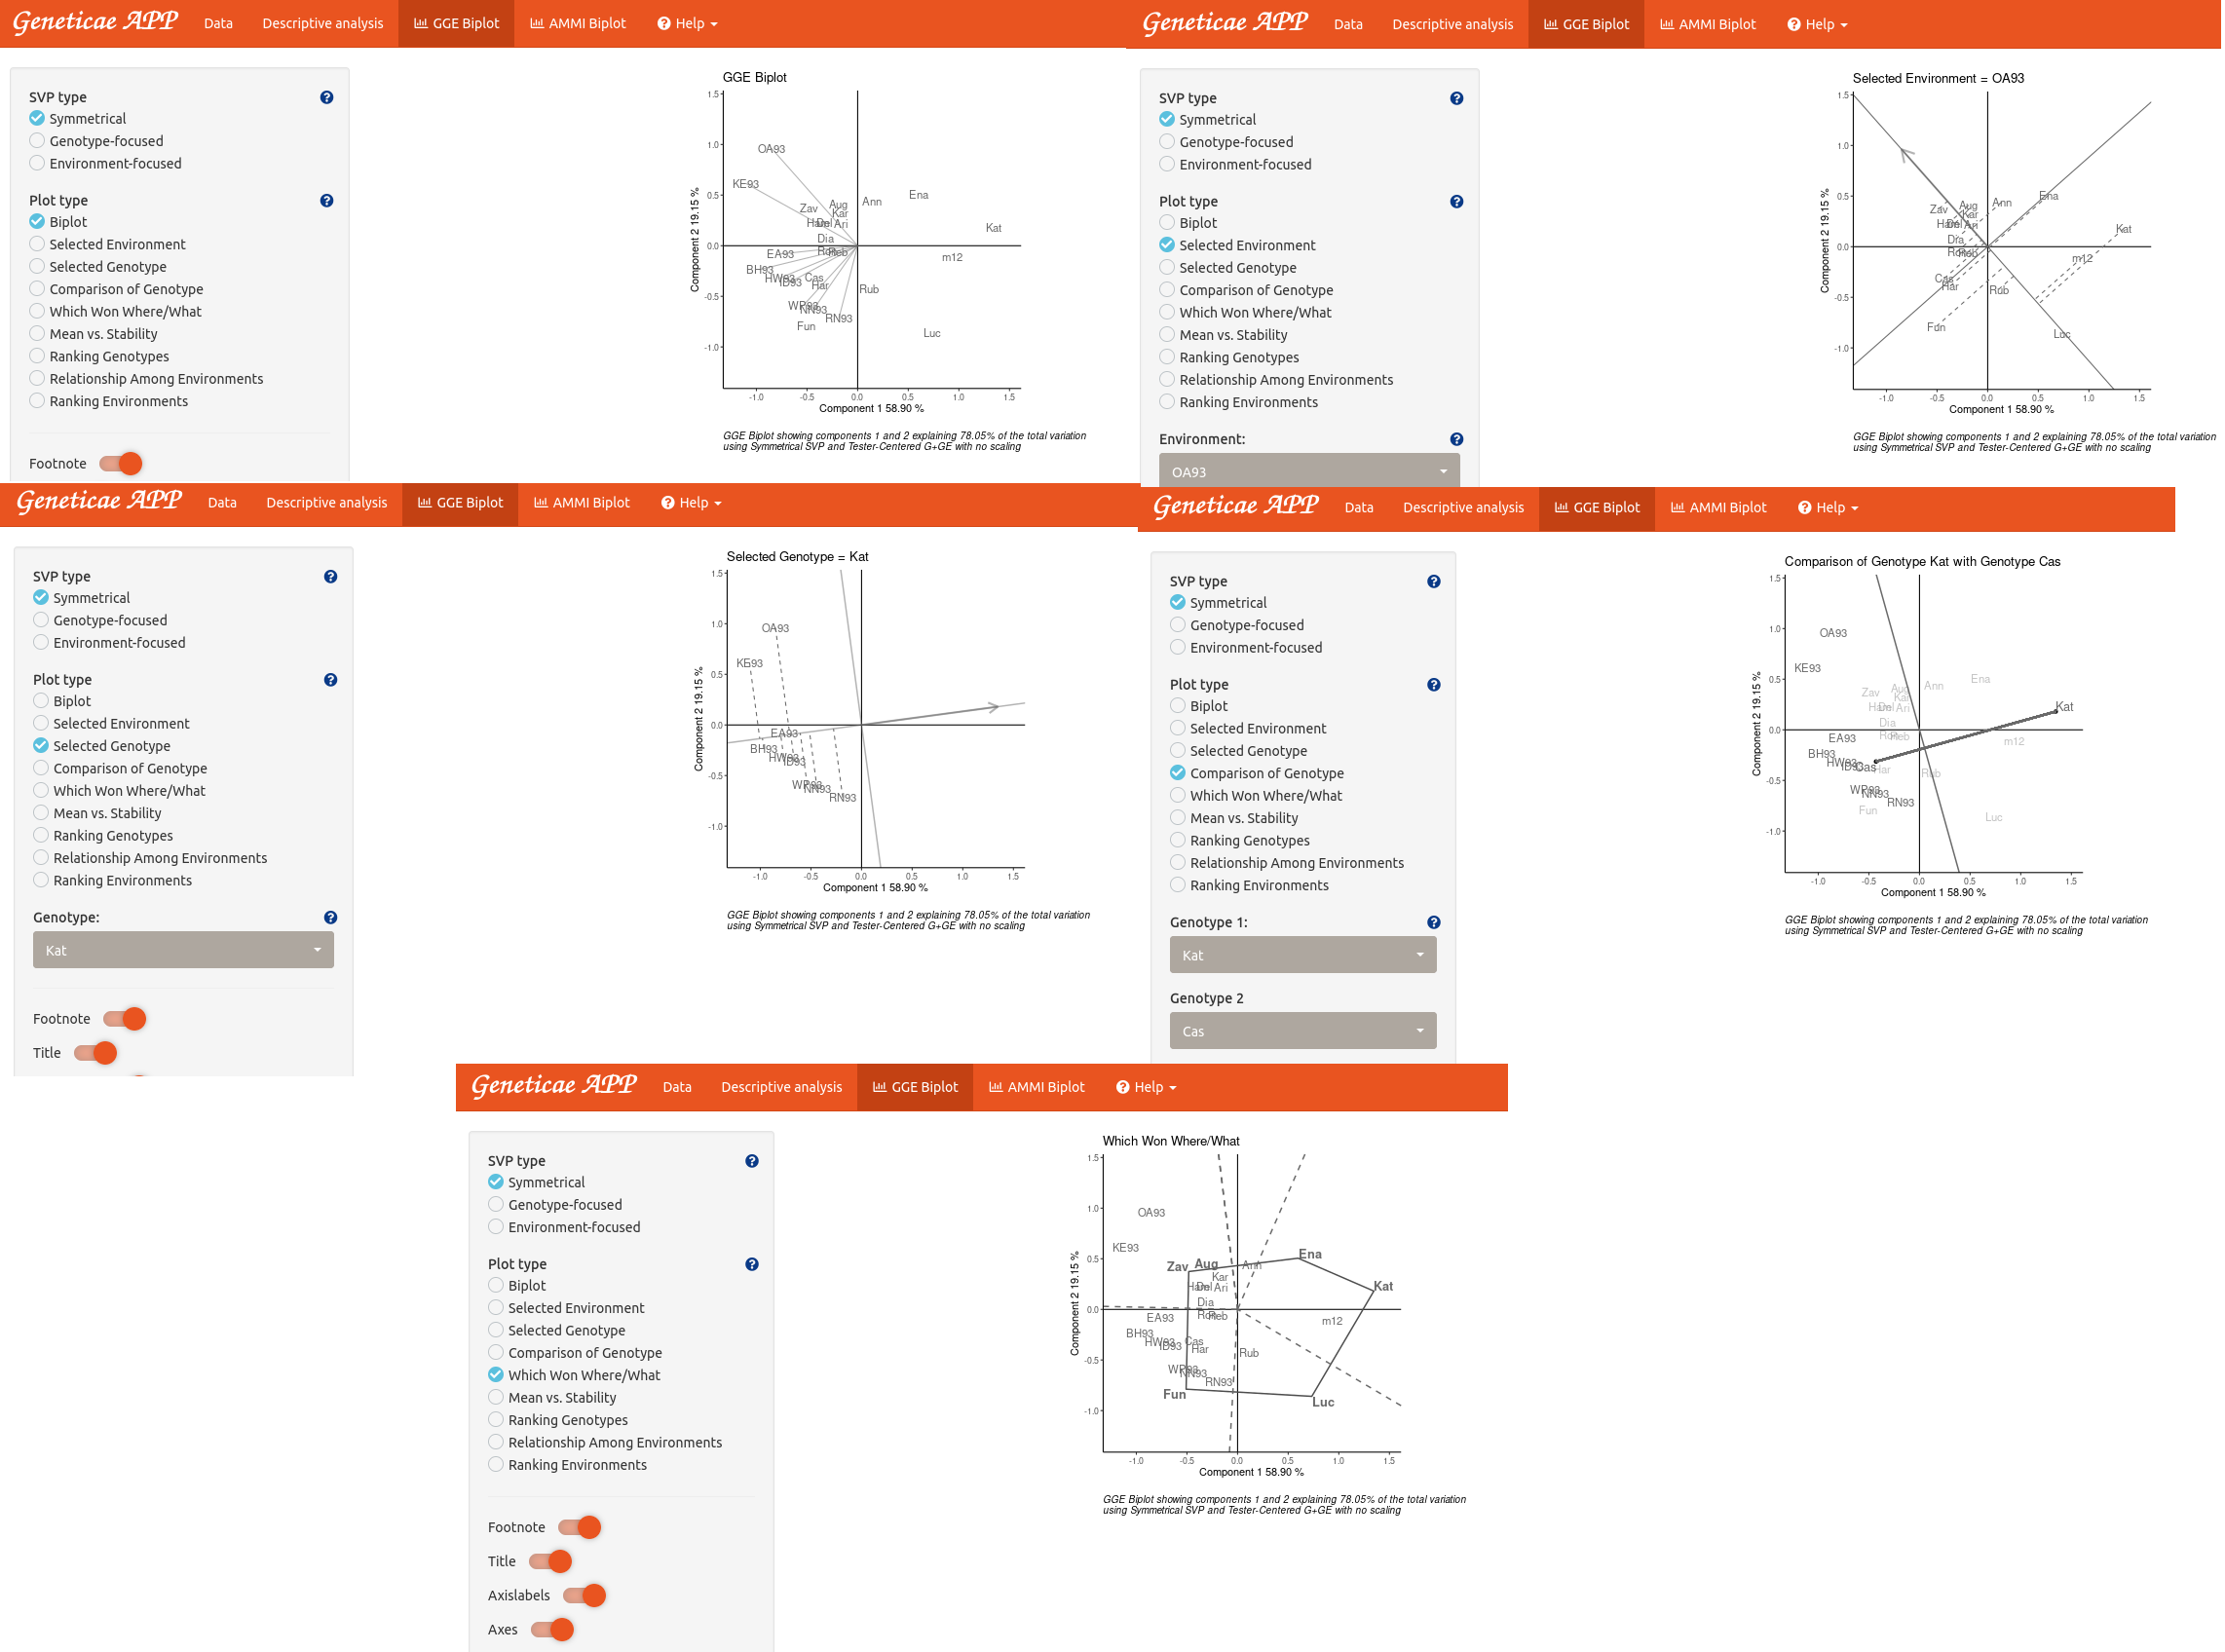
\includegraphics[width=16cm]{./Graficos/www/GGE_biplotAPP1.png}
	\end{center}
	\caption{Boxplot de genotipos a través de los ambientes para el conjunto de datos Plrv}
	\label{fig:ggebip1}
\end{figure}

La selección de cultivares dentro de cada megaambiente se realiza con la partición de valores singulares enfocada en los genotypos (\emph{SVP type $->$ genotype-focused}), y los tipos de gráficos que se pueden realizar son: \emph{Mean vs. Stability} que permite la visualización de la media y estabilidad de genotipos y \emph{Ranking Genotypes} que compara las cultivares con el ``ideal" (Figura \ref{fig:ggebip2}). Dado que estos análisis son propios de cada megaambiente, al indicar alguno de estas vistas del biplot GGE se tendrá que señalar cuales son los ambientes que forman el megaambiente de interés. 


\begin{figure}[H]
	\begin{center}
		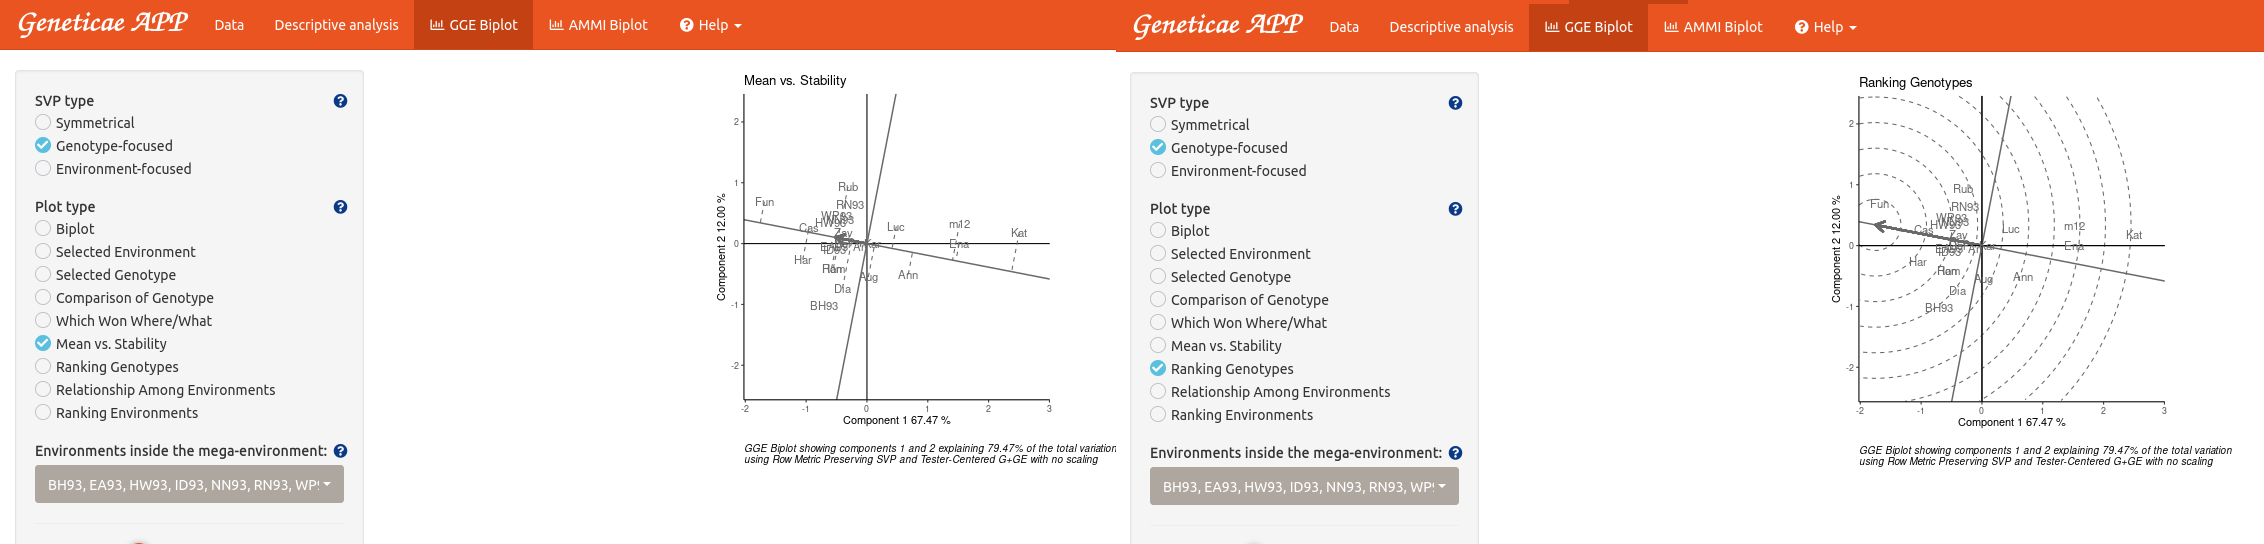
\includegraphics[width=16cm]{./Graficos/www/GGE_biplotAPP2.png}
	\end{center}
	\caption{Boxplot de genotipos a través de los ambientes para el conjunto de datos Plrv}
	\label{fig:ggebip2}
\end{figure}

Por último, para el análisis de los ambientes de cada megaambiente se utiliza el método de partición de valores singulares centrado en los ambientes (\emph{SVP type $->$ environment-focused}). Para comprender las interrelaciones entre ellos el tipo de gráfico \emph{Relationship Among Environments} se debe seleccionar y para visualizar la dapacidad de discriminación y representatividad 
\emph{Ranking Environments} (Figura \ref{fig:ggebip3}). Dado que estos análisis son propios de cada megaambiente, al indicar alguno de estas vistas del biplot GGE se tendrá que señalar cuales son los ambientes que forman el megaambiente de interés. 


\begin{figure}[H]
	\begin{center}
		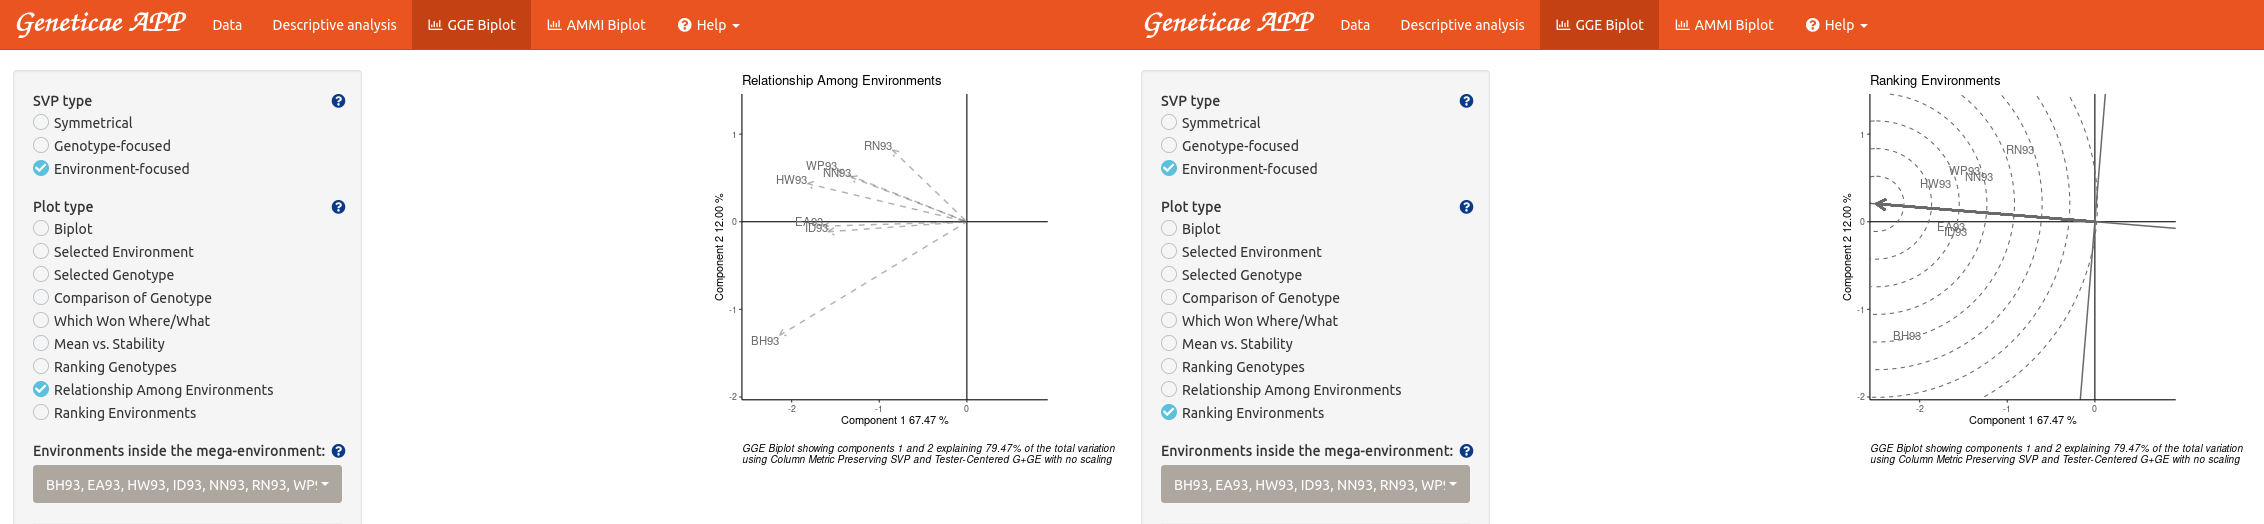
\includegraphics[width=16cm]{./Graficos/www/GGE_biplotAPP3.png}
	\end{center}
	\caption{Boxplot de genotipos a través de los ambientes para el conjunto de datos Plrv}
	\label{fig:ggebip3}
\end{figure}


\subsection{modelo AMMI}

La pestaña \emph{AMMI Biplot} crea el biplot GE, en el que los cultivares se muestran en minúsculas y los entornos en mayúsculas. Dado que las alternativas clásica y robustas requieren una única observación para cada combinación de genotipo y ambiente, si hay repeticiones, el valor promedio fenotípico se calcula automáticamente antes de ajustar el modelo. No se permiten valores perdidos. Al igual que en el biplot de GGE, una nota a pie de página que indica que el porcentaje de variación de IGA explicado por los dos ejes, el gráfico de título, los ejes y los nombres de los mismos se pueden configurar para que aparezcan o no. Además, el color y tamaño del marcador de genotipos y ambientes pueden ser personalizados por el usuario. Los biplots pueden ser descargados.

Por ejemplo, para obtener el biplot GE derivado del modelo AMMI clásico se debe indicar
AMMI en \emph{plot type} (Figura ...). En caso de contar con \emph{outliers} alguna de las alternativas robustas (rAMMI, hAMMI, gAMMI, lAMMI o ppAMMI) se debe especificar.
 

\begin{figure}[H]
	\begin{center}
		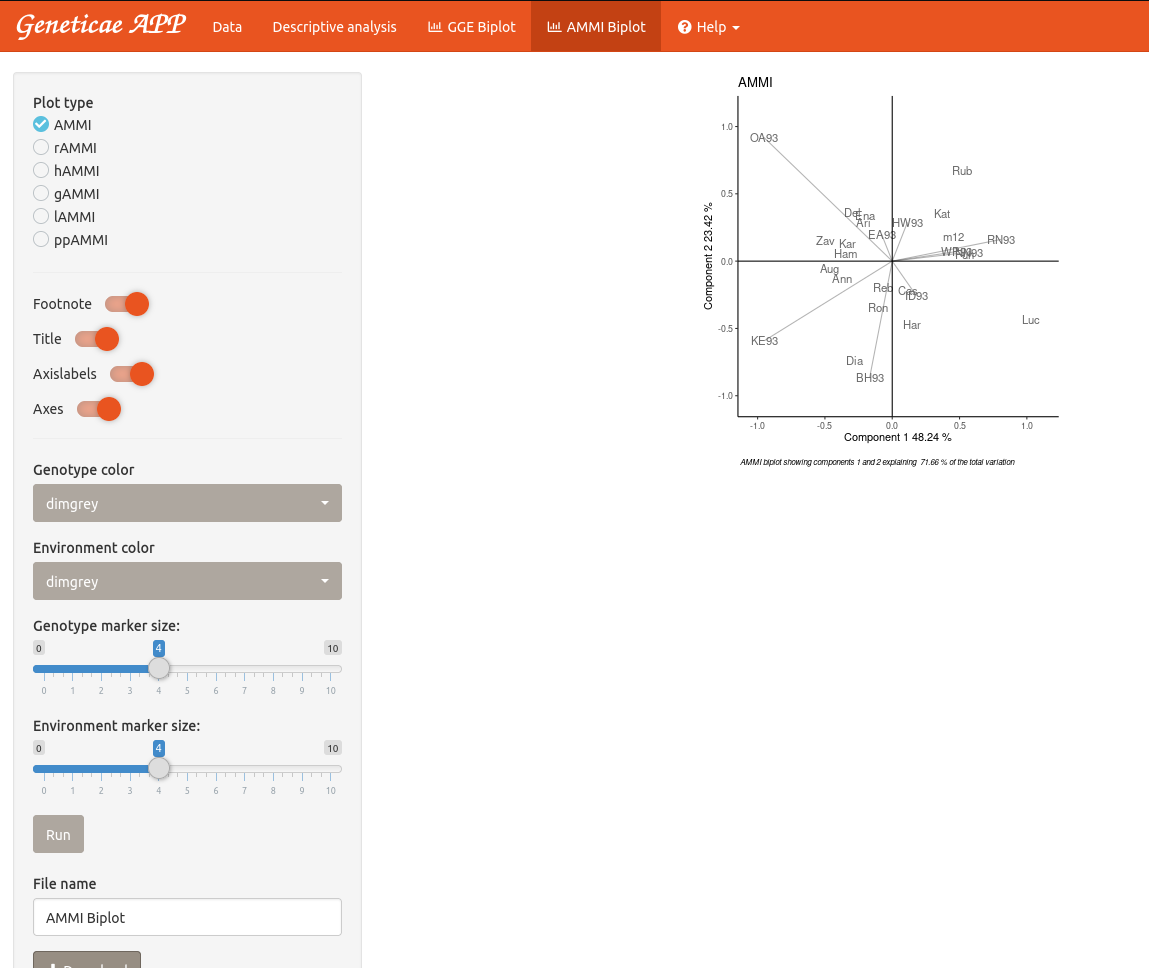
\includegraphics[width=16cm]{./Graficos/AMMI_GE.png}
	\end{center}
	\caption{AMMI}
	\label{fig:fig4313}
\end{figure}


\subsection{Ayuda}

En la pestaña \emph{Help} se presenta información general, un tutorial y un video sobre  cómo utilizar la APP.
